\subsection{Introducción:}

En este ejercicio vamos a realizar la Tabla de Descriptores Globales (GDT). Se pide que realizemos lo siguiente :

\begin{itemize}
\item [\textit{a)}] Que la tabla gdt tenga 4 segmentos, dos para código de
nivel 0 y 3; y otros dos para datos de nivel 0 y 3. Estos segmentos deben direccionar los primeros 500MB de memoria. Por último se pide no usar las primeras siete posiciones de la gdt, ya que se consideran utilizadas.

\item [\textit{b)}] Pasar a modo protegido y setear la pila del kernel en la direccion 0x27000. 

\item [\textit{c)}] Agregar a la gdt un segmento adicional y escribir una rutina qe utilice este nuevo segmento para pintar la esquina superior izquierda de la pantalla.

\item [\textit{d)}] Limpiar la pantalla y pintar el área del mapa (sugerido el color gris) junto con las barras inferiores para los jugadores.
\end{itemize}

\subsection{Ítem a: Setear la GDT}

Para este ítem completamos el archivo gdt.c proporcionado por la catedra. En el mismo la GDT es representada mediante un array de 30 posiciones. Cada posicion tiene la siguiente estructura.
\\

\begin{figure}[H]
\begin{center}
\minipage{0.6\textwidth}
  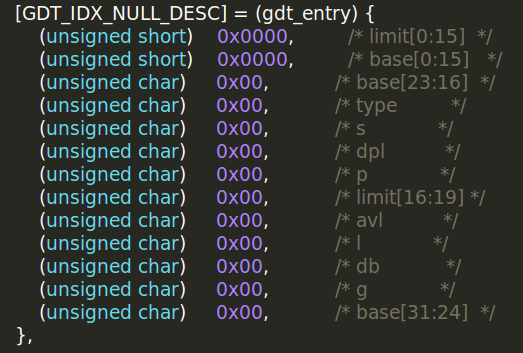
\includegraphics[width=\linewidth]{ejercicio1/GDTnula.png}
  \caption{{\small Este descriptor corresponde a la primer entrada de la gdt}} 
\endminipage
\end{center}
\end{figure}

Como la primer posicion de la tabla GDT debe ser corresponder a una entrada nula, llenamos la primer posicion como muestra la imagen debajo.
\\

\begin{figure}[H]
\begin{center}
\minipage{0.55\textwidth}
  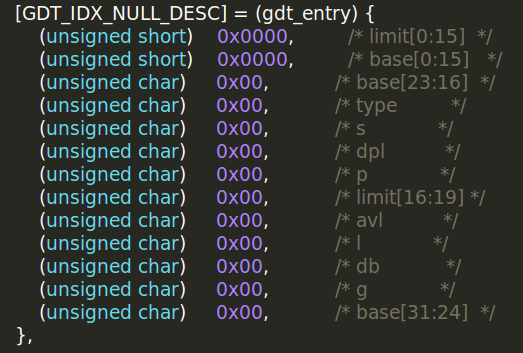
\includegraphics[width=\linewidth]{ejercicio1/GDTnula.png}
  \caption{{\small Este descriptor corresponde a la primer entrada de la gdt}} 
\endminipage
\end{center}
\end{figure}

Luego, creamos los 4 segmentos que se piden a partir de la posicion 8 de la GDT, ya que por enunciado, no se deben tocar las primeras 7 posiciones de la table de descriptores. Mostramos en las imagenes de abajo como creamos un descriptor de datos y otro de codigos. 
\\

\begin{figure}[H]
\begin{center}
\minipage{0.5\textwidth}
  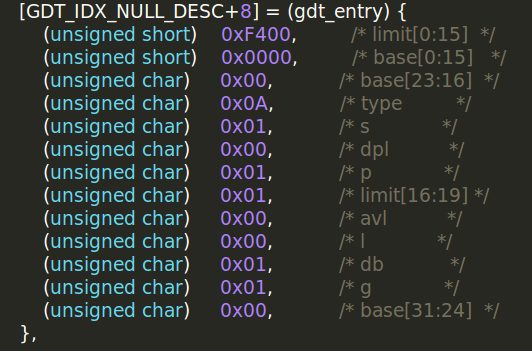
\includegraphics[width=\linewidth]{ejercicio1/GDTcodigo0.png}
  \caption{{\small Este descriptor corresponde al segmento de datos de nivel 0}} 
\endminipage
\minipage{0.5\textwidth}
  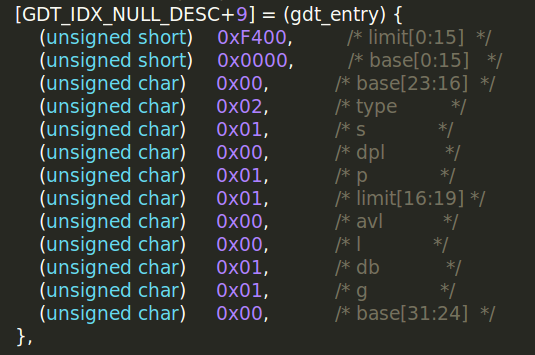
\includegraphics[width=\linewidth]{ejercicio1/GDTdatos0.png}
  \caption{{\small Este descriptor corresponde al segmento de código de nivel 0}} 
\endminipage
\end{center}
\end{figure}

Los otros dos que faltan son exactamente iguales, solo que en la linea correspondiente al nivel (dpl) ponemos 0x03, ya que corresponde al nivel 3 de prioridad.
\\

Los descriptores de segmentos tienen la siguiente forma:
\\

\begin{figure}[H]
\begin{center}
\minipage{0.8\textwidth}
  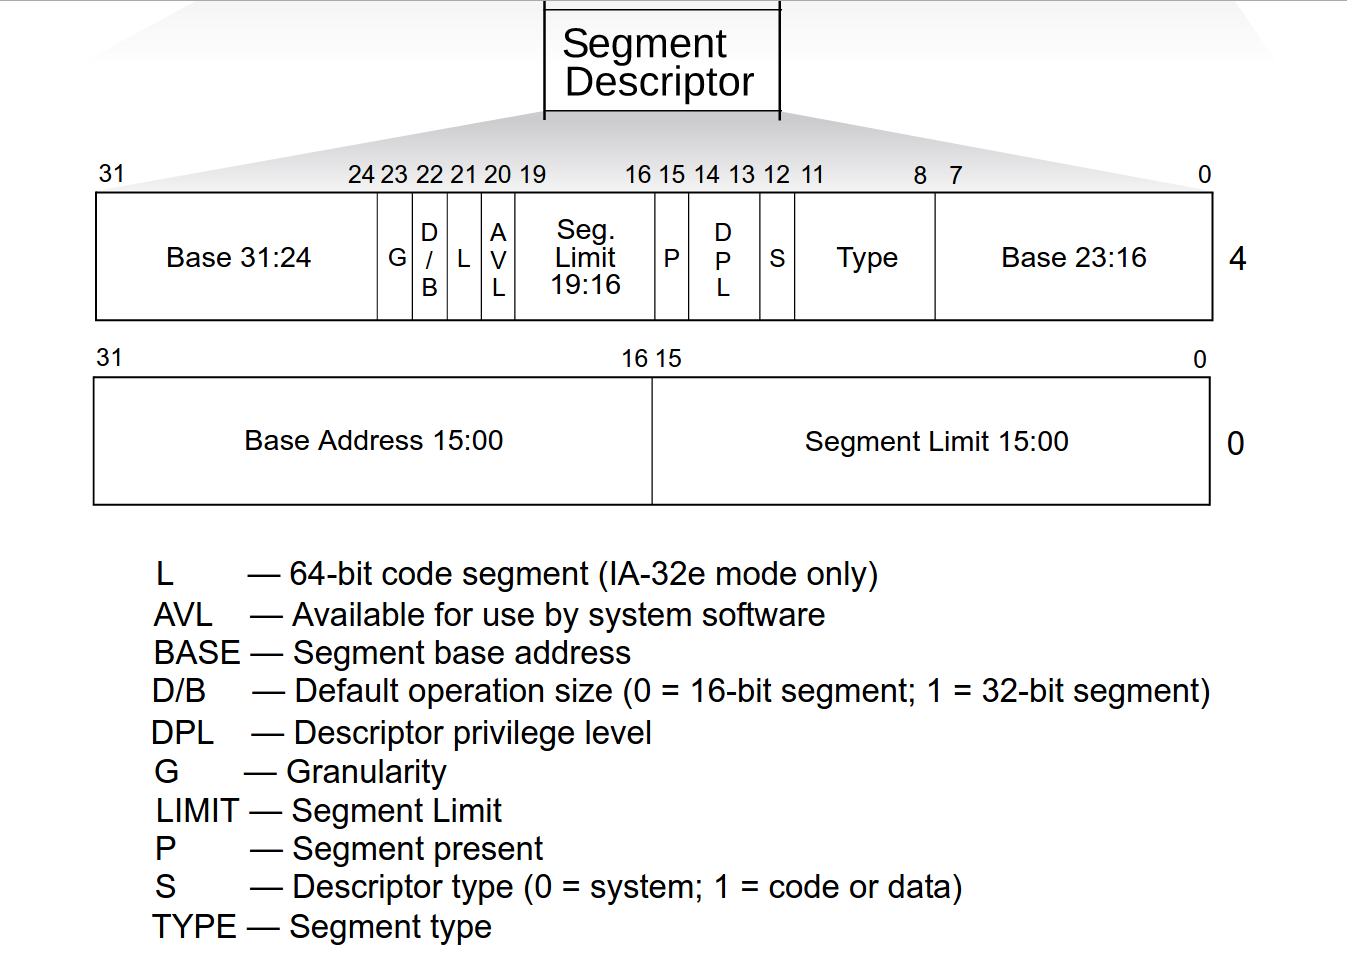
\includegraphics[width=\linewidth]{ejercicio1/estructuradescriptor.png}
  \caption{{\small Este descriptor corresponde a la primer entrada de la gdt}} 
\endminipage
\end{center}
\end{figure}

Completamos nuestros descriptores como marcan las figuras 3 y 4 de esa forma porque:

\begin{itemize}
\item [\textit{Base:}] En el tp se pide que los descriptores direcciones los primeros 500mb de memoria. Por ende la base corresponde a la direccion 0x00000000.
\item [\textit{G:}]  Para poder direccionar 500mb, no nos alcanza la cantidad de bits que hay para el limite, por ende necesitamos activar la granularidad para poder abarcar más memoria, ya que cuando esta activada la posicion que indica el limite se multiplica por 4kb.
\item [\textit{Límite:}] Como esta activada la granularidad, podemos abarcar 500mb de memoria, el limite correspondiente a 500mb con la granularidad activada es 0x0F400.
\item [\textit{Type:}] Aqui se indica si el descriptor es de código/datos, a los correspondientes a datos les pusimos que eran de tipo 0x02 (segmento de datos de escritura/lectura) y a los de codigo que eran de tipo 0x0A (segmentdo de código de escritura/lectura).
\item [\textit{S:}] Con este bit se decide si es un segmento de sistema (s=0) o si son de código/data (s=1), por ende a este bit le corresponde un 0x1.
\item [\textit{Dpl:}] En esta seccion se declara el privilegio del segmento, a los que eran de nivel 0 les corresponde un 0x00 y a los de nivel 3 un 0x03
\item [\textit{P:}] Este es el bit de present. Cuando es ’1’ el segmento correspondiente esta presente en la memoria RAM. Si es ’0’, el segmento esta en la memoria virtual. Por ende lo seteamos en 1.
\item [\textit{Avl:}] Es el bit correspondiente a Available. Como no lo vamos a tener en cuenta lo dejamos en 0.
\item [\textit{L:}] Indica si el codigo es de 64bits o de 32. Como trabajamos en 32bits dejamos este bit en 0.
\item [\textit{D/B:}] Este bit define el tamaño de las operaciones en las que va a trabajar el procesador. De nuevo, como nos encontramos trabajando en 32bits, el tamaño de las operaciones debe ser de 32, por eso lo seteamos en 1.
\end{itemize}

\subsection{Ítem B: Pasar a modo protegido y setear la pila}









